% !TEX program = xelatex
% !TEX options = --shell-escape
\documentclass[a4paper,9]{article}
\usepackage{zh_CN-Adobefonts_external} % Simplified Chinese Support using external fonts (./fonts/zh_CN-Adobe/)
\usepackage{fancyhdr}
\usepackage[cache=false]{minted}
\usemintedstyle{bw}
\usepackage[colorlinks]{hyperref}
\setlength{\headheight}{15pt}
\usepackage{geometry}
\usepackage{amsmath,amssymb,bm}
\usepackage{pdfpages}

% 定义页边距
\geometry{a4paper,left=1cm,right=1cm,top=2cm,bottom=2cm}

% 定义页眉页脚
\pagestyle{fancy}
\fancyhf{}
\fancyhead[C]{Algorithm Library by nickluo}
\lfoot{}
\cfoot{\thepage}
\rfoot{}

\author{nickluo}
\title{Algorithm Library\footnote{The template of these templates is based on the \href{https://github.com/palayutm/ply-template}{ply-template} by \href{https://github.com/palayutm}{palayutm}}}

\begin{document}

\twocolumn  % 分页显示

\maketitle % 封面
% \newpage % 换页
\tableofcontents % 目录

\section{vimrc}
\inputminted[breaklines]{vim}{vimrc/vimrc}

\section{Z}
\inputminted[breaklines]{c++}{Z/z.cpp} % 插入代码文件

\section{随机数生成器}
\inputminted[breaklines]{c++}{random/rand_gen.cpp}

\section{数列与计数}
\subsection{多项式板子}
\inputminted[breaklines]{c++}{sequence/polynomial.cpp}
\subsection{牛顿迭代}
\noindent \textbf{问题描述:}给出多项式$G(x)$,求解多项式$F(x)$满足:
\[G(F(x)) \equiv 0 \pmod {x^n}\]
答案只需要精确到$F(x) \bmod {x^n}$即可。\par
\noindent \textbf{实现原理:}考虑倍增,假设有:
\[G(F_t(x)) \equiv 0 \pmod{x^t}\]
对$G(F_{t + 1}(x))$在模$x^{2t}$意义下进行Taylor展开:
\[G(F_{t + 1}(x)) \equiv G(F_t(x)) + \dfrac{G'(F_t(x))}{1!}(F_{t + 1}(x) - F_t(x)) \pmod{x^{2t}}\]
那么就有:
\[F_{t + 1}(x) \equiv F_t(x) - \dfrac{G(F_t(x))}{G'(F_t(x))} \pmod{x^{2t}}\]
\noindent \textbf{注意事项:}$G(F(x))$的常数项系数必然为0,这个可以作为求解的
初始条件。
\par
\noindent \textbf{多项式求逆}
\noindent \textbf{原理:}令$G(x) = x * A - 1$(其中$A$是一个多项式系数),根据牛顿迭代法有:
\begin{displaymath}
\begin{split}
F_{t + 1}(x) &\equiv F_t(x) - \dfrac{F_t(x) * A(x) - 1}{A(x)} \\
&\equiv 2F_t(x) - F_t(x)^2 * A(x)\pmod{x^{2t}}
\end{split}
\end{displaymath}
\noindent \textbf{注意事项:}
\begin{enumerate}
	\item $F(x)$的常数项系数必然不为0,否则没有逆元;
	\item 复杂度是$O(n \log n)$但是常数比较大($10^5$大概需要0.3秒左右);
	\item 传入的两个数组必须不同,但传入的次数界没有必要是2的次幂;
\end{enumerate}
\textbf{多项式取指数和对数}
\noindent \textbf{作用:}给出一个多项式$A(x)$,求一个多项式$F(x)$满足$e^A(x) - F(x) \equiv 0 \pmod{x^n}$。\par
\noindent \textbf{原理:}令$G(x) = \ln x - A$(其中$A$是一个多项式系数),根据牛顿迭代法有:
\[F_{t + 1}(x) \equiv F_t(x) - F_t(x)(\ln {F_t(x)} - A(x)) \pmod{x^{2t}}\]
求$\ln {F_t(x)}$可以用先求导再积分的办法,即:
\[\ln A(x) = \int \dfrac{F'(x)}{F(x)}~\mathrm{d}x\]
多项式的求导和积分可以在$O(n)$的时间内完成,因此总复杂度为$O(n \log n)$。\par
\noindent \textbf{应用:}加速多项式快速幂。\par
\noindent \textbf{注意事项:}
\begin{enumerate}
	\item 进行$\log$的多项式必须保证常数项系数为1,否则必须要先求出$\log a[0]$是多少;
	\item 传入的两个数组必须不同,但传入的次数界没有必要是2的次幂;
	\item 常数比较大,$10^5$的数据求指数和对数分别需要0.37s和0.85s左右的时间,注意这里{memset}几乎不占用时。
\end{enumerate}

\subsection{MTT}
\inputminted[breaklines]{c++}{sequence/mtt.cpp}
\subsection{FWT}
\inputminted[breaklines]{c++}{sequence/fwt.cpp}
\subsection{BM}
\inputminted[breaklines]{c++}{sequence/bm.cpp}
\subsection{numbers}
\subsubsection{伯努利数}
\noindent 伯努利数满足
\begin{equation*}
    B_0 = 1, \sum_{j=0}^m \binom{m+1}{j} B_j = 0 ~ (m > 0).
\end{equation*}
\noindent 等式两边同时加上 $B_{m+1}$,并设 $n = m - 1$,得
\begin{equation*}
\sum_{i=0}^n \binom{n}{i} = [n = 1] + B_n
\end{equation*}
\noindent 设 $\hat{B}(x) = \sum_{i=0}^\infty B_i \cdot \frac{x^i}{i!}$,则
\begin{equation*}
\hat{B}(x) e^x = x + \hat{B}(x) \Rightarrow \hat{B}(x) = \frac{x}{e^x - 1} \\
\end{equation*}
\begin{equation*}
\begin{aligned}
& 0^k + 1^k + \ldots + n^k \\
=& ~ k! [x^k] \frac{e^{(n+1)x}-1}{x} \cdot \hat{B}(x) \\
=& ~ k! \sum_{i=0}^k \frac{B_i}{i!} \cdot \frac{(n+1)^{k-i+1}}{(k-i+1)!} \\
=& ~ \frac{1}{k+1} \sum_{i=0}^k \binom{k+1}{i} B_i \cdot (n+1)^{k-i+1}
\end{aligned}
\end{equation*}

\subsubsection{第一类斯特林数}
\noindent 记 $S_1(n, k)$ 为将 $n$ 个不同元素分为 $k$ 个环排列的方案数. 由组合意义得,
$$
S_1(n, k) = S_1(n - 1, k - 1) + (n - 1) S_1(n - 1, k)
$$
$$
x^{\overline{n}} = \sum_{i=0}^n S_1(n, i) x^i
$$
$$
x^{\underline{n}} = \sum_{i=0}^n (-1)^{n-i} S_1(n, i) x^i
$$
$$
\sum_{i=0}^n S_1(n, i) x^i = \prod_{i=0}^{n-1} (x+i)
$$

\noindent 注意最后等式的右半部分,可以使用递增 + 点值平移 $O(n \log n)$ 求出第
$n$ 行斯特林数.

\subsubsection{第二类斯特林数}
\noindent 记 $S_2(n, k)$ 为将 $n$ 个不同元素分至 $k$ 个相同的盒子(每个盒子至
少一个元素)的方案数. 由组合意义得,
$$
S_2(n, k) = S_2(n - 1, k - 1) + k S_2(n - 1, k)
$$
$$
x^n = \sum_{i=0}^n S_2(n, i) x^{\underline{i}}
$$
$$
S_2(n, k) = \sum_{i=0}^k (-1)^{k-i} \binom{k}{i} i^n
$$
$$
\frac{S_2(n, k)}{k!} = \sum_{i=0}^k \frac{i^n}{i!} \cdot \frac{(-1)^{k-i}}
{(k-i)!}
$$
\noindent 是一个卷积的形式,可以 FFT 求出某一行第二类斯特林数.

\subsubsection{斯特林反演}
\begin{equation*}
    \begin{aligned}
        x^n &= \sum_{i=0}^n S_2(n, i) x^{\underline{i}} \\
        &= \sum_{i=0}^n S_2(n, i) \sum_{j=0}^i (-1)^{i-j} S_1(i, j) x^j \\
        &= \sum_{i=0}^n x^i \sum_{j=i}^n (-1)^{j-i} S_2(n, j) S_1(j, i)
    \end{aligned}
\end{equation*}
\noindent 设
\begin{equation*}
    g_n = \sum_{i=0}^n S_2(n, i) f_i,
\end{equation*}
\noindent 则
\begin{equation*}
    f_n = \sum_{i=0}^n (-1)^{n-i} S_1(n, i) g_i.
\end{equation*}

\subsubsection{Burnside 引理}
设置换群为 $G$,染色集合为 $X$.

若染色 $x \in X$ 在置换 $f$ 的作用下得到染色 $y \in X$,则称 $x, y$ 等价.
由置换群的定义,我们可以得到等价类,使得等价类内任意两个染色等价.

设 $X^g (g \in G)$ 表示在置换 $g$ 下的不动点,即
$$
X^g = \{x \mid x \in X, gx = x\}.
$$
则等价类个数
$$
|X / G| = \frac{1}{|G|} \sum_{g \in G} |X^g|.
$$

例 LOJ 6538 烷基计数,对于一棵有根树,每个节点至多三个儿子,且这些儿子排列同
构. 求有多少个 $n$ 个节点的等价类.

考虑其生成函数 $f(x)$.
根节点有 $3$ 个儿子(儿子可以为空,因为循环同构,我们不需讨论 $0, 1, 2$ 个儿子
的情况),排列的置换群有 $6$ 种,其中 $(1,2,3)$ 染色方案数为 $f(x)^3$,
$(1,3,2),(2,1,3),(3,2,1)$ 染色方案为 $f(x^2)f(x)$,$(2,3,1),(3,1,2)$ 染色方案
为 $f(x^3)$. 所以
$$
f(x) = x \times \frac{f(x)^3+3f(x^2)f(x)+2f(x^3)}{6}+1.
$$
牛顿迭代.

\subsection{树的计数}
\begin{enumerate}
	\item 有根树计数:$n+1$个结点的有根树的个数为
	$$a_{n+1} = \frac{\sum_{j=1}^{n}{j \cdot a_j \cdot{S_{n, j}}}}{n}$$
	其中,
	$$S_{n, j} = \sum_{i=1}^{n/j}{a_{n+1-ij}} = S_{n-j, j} + a_{n+1-j}$$
	\item 无根树计数:当$n$为奇数时,$n$个结点的无根树的个数为
	$$a_n-\sum_{i=1}^{n/2}{a_ia_{n-i}}$$
	当$n$为偶数时,$n$个结点的无根树的个数为
	$$a_n-\sum_{i=1}^{n/2}{a_ia_{n-i}}+\frac{1}{2}a_{\frac{n}{2}}(a_{\frac{n}{2}}+1)$$
	\item $n$个结点的完全图的生成树个数为
	$$n^{n-2}$$
	\item 矩阵-树定理:图$G$由$n$个结点构成,设$\bm{A}[G]$为图$G$的邻接矩阵、$\bm{D}[G]$为图$G$的度数矩阵,则图$G$的不同生成树的个数为$\bm{C}[G] = \bm{D}[G] - \bm{A}[G]$的任意一个$n-1$阶主子式的行列式值。
\end{enumerate}



\section{数论}
\subsection{判素数(miller-rabin)}
\inputminted[breaklines]{c++}{number_theory/miller_rabin.cpp}
\subsection{二次剩余(Cipolla)}
欧拉判定:
\begin{equation*}
    x^{\frac{p-1}{2}} \equiv \binom{\underline{x}}{p} \pmod p
\end{equation*}

\inputminted[breaklines]{c++}{number_theory/cipolla.cpp}
\subsection{杜教筛}
\inputminted[breaklines]{c++}{number_theory/dujiaoshai.cpp}
\subsection{min\_25}
\inputminted[breaklines]{c++}{number_theory/min25.cpp}
\subsection{直线下整点个数}
\inputminted[breaklines]{c++}{number_theory/lattice_count.cpp}
\subsection{定理}
\subsubsection{扩展欧拉定理}
\begin{equation*}
    a^b \equiv \begin{cases} a^{b \bmod \varphi(m)} & (\gcd(a, m) = 1) \\ a^b & (\gcd(a, m) \ne 1, b < \varphi(m)) \\ a^{(b \bmod \varphi(m)) + \varphi(m)} & (\gcd(a, m) \ne 1, b \ge \varphi(m)) \end{cases} \pmod m
\end{equation*}

\subsubsection{卢卡斯定理}
\noindent $\forall$ 质数 $p, n, m \in \mathbb{N}^{+}$,
\begin{equation*}
    \binom{n}{m} \equiv \binom{\lfloor n/p \rfloor}{\lfloor m/p \rfloor}
    \binom{n \bmod p}{m \bmod p} \pmod p
\end{equation*}

\subsubsection{威尔逊定理}
\noindent 对于质数 $p$,有 $(p-1)! \equiv -1 \pmod p$(证明 $2, 3, \ldots, p -
2$ 可以逆元两两配对)
\noindent 高斯的扩展:
\begin{equation*}
    \prod_{1 \le k \le m, \gcd(k, m) = 1} k \equiv \begin{cases} -1, &
    \text{if } m = 4, p^\alpha, 2p^\alpha, \\ 1, & \text{otherwise}. \end{cases}
    \pmod m
\end{equation*}


\section{线性代数}
\subsection{线性基}
\inputminted[breaklines]{c++}{linear_algebra/lb.cpp}
\subsection{矩阵求逆}
\inputminted[breaklines]{c++}{linear_algebra/matrix_inversion.cpp}
\subsection{矩阵特征多项式}
\inputminted[breaklines]{c++}{linear_algebra/charac-poly.cpp}

\section{数据结构}
\subsection{左偏树}
\inputminted[breaklines]{c++}{data_structure/leftist_tree.cpp}
\subsection{LCT}
\inputminted[breaklines]{c++}{data_structure/lct.cpp}
\subsection{KD-Tree}
\inputminted[breaklines]{c++}{data_structure/kd_tree.cpp}

\section{图论}
\subsection{点双}
\inputminted[breaklines]{c++}{graph/bcc.cpp}
\subsection{全局平衡二叉树}
\inputminted[breaklines]{c++}{graph/全局平衡二叉树.cpp}
\subsection{求欧拉回路}
\inputminted[breaklines]{c++}{graph/euler_tour.cpp}
\subsection{SPFA}
\inputminted[breaklines]{c++}{graph/spfa.cpp}
\subsection{虚树}
\inputminted[breaklines]{c++}{graph/xushu.cpp}
\subsection{2-SAT}
\inputminted[breaklines]{c++}{graph/2_sat.cpp}
\subsection{有根树同构}
\inputminted[breaklines]{c++}{graph/rooted_tree_isom.cpp}
\subsection{支配树}
\inputminted[breaklines,breakanywhere]{c++}{graph/dominator.cpp}
\subsection{MCS 求 PEO}
\inputminted[breaklines]{c++}{graph/MCS.cpp}
\subsection{最大团}
\inputminted[breaklines]{c++}{graph/maximum-clique.cpp}
\subsection{最小树形图}
\inputminted[breaklines]{c++}{graph/dmst.cpp}
\subsection{二分图最大权匹配(KM)}
\inputminted[breaklines]{c++}{graph/KM.cpp}
\subsection{一般图最大权匹配}
\inputminted[breaklines,breakanywhere]{c++}{graph/blossom.cpp}
\subsection{无向图最小割}
\inputminted[breaklines,breakanywhere]{c++}{graph/mincut.cpp}

\section{字符串}
\subsection{后缀树组}
\inputminted[breaklines]{c++}{string/sa.cpp}
\subsection{后缀自动机}
\inputminted[breaklines]{c++}{string/sam.cpp}
\subsection{Manacher}
\inputminted[breaklines]{c++}{string/manacher.cpp}
\subsection{回文自动机}
\inputminted[breaklines]{c++}{string/pam.cpp}
\subsection{Lyndon 分解}
\inputminted[breaklines]{c++}{string/lyndon.cpp}
\subsection{Z Function}
\inputminted[breaklines]{c++}{string/z_func.cpp}

\section{计算几何}
\subsection{基本操作}
\inputminted[breaklines]{c++}{geometry/basic.cpp}
\subsection{半平面交}
\inputminted[breaklines]{c++}{geometry/half-plane-intersection.cpp}
\subsection{凸包操作}
\inputminted[breaklines]{c++}{geometry/convex.cpp}
\subsection{动态维护凸壳}
\inputminted[breaklines]{c++}{geometry/dynamic-convex.cpp}

\section{其他}
\subsection{网络流(ISAP)}
\inputminted[breaklines]{c++}{others/isap.cpp}
\subsection{网络流(HLPP)}
\inputminted[breaklines]{c++}{others/hlpp.cpp}
\subsection{最小费用流}
\inputminted[breaklines,breakanywhere]{c++}{others/mincost.cpp}
\subsection{模拟退火}
\inputminted[breaklines]{c++}{others/simulate_anneal.cpp}
\subsection{Simpson 积分}
\inputminted[breaklines]{c++}{others/simpson.cpp}
\subsection{线性规划}
\inputminted[breaklines]{c++}{others/linear-programming.cpp}
\subsection{积分表}
\begin{footnotesize}
\noindent
\mbox{\vbox to 11pt{  \hbox{$
\int \frac{1}{1+x^2}dx = \tan^{-1}x
$}  }}
\
\mbox{\vbox to 11pt{  \hbox{$
\int \frac{1}{a^2+x^2}dx = \frac{1}{a}\tan^{-1}\frac{x}{a}
$}  }}
\\
\mbox{\vbox to 11pt{  \hbox{$
\int \frac{x}{a^2+x^2}dx = \frac{1}{2}\ln|a^2+x^2|
$}  }}
\
\mbox{\vbox to 11pt{  \hbox{$
\int \frac{x^2}{a^2+x^2}dx = x-a\tan^{-1}\frac{x}{a}
$}  }}
\\
\mbox{\vbox to 11pt{  \hbox{$
\int\sqrt{x^2 \pm a^2} dx  = \frac{1}{2}x\sqrt{x^2\pm a^2}
%\nonumber \\
\pm\frac{1}{2}a^2 \ln \left | x + \sqrt{x^2\pm a^2} \right |
$}  }}
\\
\mbox{\vbox to 11pt{  \hbox{$
\int  \sqrt{a^2 - x^2} dx  = \frac{1}{2} x \sqrt{a^2-x^2}
%\nonumber \\
+\frac{1}{2}a^2\tan^{-1}\frac{x}{\sqrt{a^2-x^2}}
$}  }}
\\
\mbox{\vbox to 11pt{  \hbox{$
\int \frac{x^2}{\sqrt{x^2 \pm a^2}} dx  = \frac{1}{2}x\sqrt{x^2 \pm a^2}
%\nonumber \\
\mp \frac{1}{2}a^2 \ln \left| x + \sqrt{x^2\pm a^2} \right |
$}  }}
\\
\mbox{\vbox to 11pt{  \hbox{$
\int \frac{1}{\sqrt{x^2 \pm a^2}} dx = \\ \ln \left | x + \sqrt{x^2 \pm a^2} \right |
$}  }}
\\
\mbox{\vbox to 11pt{  \hbox{$
\int \frac{1}{\sqrt{a^2 - x^2}} dx = \sin^{-1}\frac{x}{a}
$}  }}
\\
\mbox{\vbox to 11pt{  \hbox{$
\int \frac{x}{\sqrt{x^2\pm a^2}}dx = \sqrt{x^2 \pm a^2}
$}  }}
\\
\mbox{\vbox to 11pt{  \hbox{$
\int \frac{x}{\sqrt{a^2-x^2}}dx = -\sqrt{a^2-x^2}
$}  }}
\\
\mbox{\vbox to 11pt{  \hbox{$
\int  \sqrt{a x^2 + b x + c} dx =
\frac{b+2ax}{4a}\sqrt{ax^2+bx+c}
\nonumber \\
+
$}  }}
\\
\mbox{\vbox to 11pt{  \hbox{$
    \text{          } \frac{4ac-b^2}{8a^{3/2}}\ln \left| 2ax + b + \\ 2\sqrt{a(ax^2+bx^+c)}\right |
$}  }}
\\
\mbox{\vbox to 11pt{  \hbox{$
\int x^n e^{ax}\hspace{1pt}\text{d}x = \dfrac{x^n e^{ax}}{a} -
\dfrac{n}{a}\int x^{n-1}e^{ax}\hspace{1pt}\text{d}x
$}  }}
\\
\mbox{\vbox to 11pt{  \hbox{$
\int \sin^2 ax dx = \frac{x}{2} - \frac{1} {4a} \sin{2ax}
$}  }}
\
\mbox{\vbox to 11pt{  \hbox{$
\int \sin^3 ax dx = -\frac{3 \cos ax}{4a} + \frac{\cos 3ax} {12a}
$}  }}
\\
\mbox{\vbox to 11pt{  \hbox{$
\int \cos^2 ax dx = \frac{x}{2}+\frac{ \sin 2ax}{4a}
$}  }}
\
\mbox{\vbox to 11pt{  \hbox{$
\int \cos^3 ax dx = \frac{3 \sin ax}{4a}+\frac{ \sin 3ax}{12a}
$}  }}
\\
\mbox{\vbox to 11pt{  \hbox{$
\int \tan ax dx = -\frac{1}{a} \ln \cos ax
$}  }}
\
\mbox{\vbox to 11pt{  \hbox{$
\int \tan^2 ax dx = -x + \frac{1}{a} \tan ax
$}  }}
\\
\mbox{\vbox to 11pt{  \hbox{$
\int x \cos ax dx = \frac{1}{a^2} \cos ax + \frac{x}{a} \sin ax
$}  }}
\
\mbox{\vbox to 11pt{  \hbox{$
\int x^2 \cos ax dx = \frac{2 x \cos ax }{a^2} + \frac{ a^2 x^2 - 2  }{a^3} \sin ax
$}  }}
\\
\mbox{\vbox to 11pt{  \hbox{$
\int x \sin ax dx = -\frac{x \cos ax}{a} + \frac{\sin ax}{a^2}
$}  }}
\
\mbox{\vbox to 11pt{  \hbox{$
\int x^2 \sin ax dx =\frac{2-a^2x^2}{a^3}\cos ax +\frac{ 2 x \sin ax}{a^2}
$}  }}
\end{footnotesize}

\subsection{Dreadnought}
\subsubsection{弦图}
设 $next(v)$ 表示 $N(v)$ 中最前的点 .
令 $w*$ 表示所有满足 $A \in B$ 的 $w$ 中最后的一个点 ,
判断 $v \cup N(v)$ 是否为极大团 ,
只需判断是否存在一个 $w \in w*$,
满足 $Next(w)=v$ 且 $|N(v)| + 1 \leq |N(w)|$ 即可 .
\subsubsection{五边形数}
$
    \prod_{n=1}^{\infty}{(1-x^{n})}=\sum_{n=0}^{\infty}{(-1)^{n}(1-x^{2n+1})x^{n(3n+1)/2}}
$
\subsubsection{重心}
半径为 $r$ , 圆心角为 $\theta$ 的扇形重心与圆心的距离为 $\frac{4r\sin(\theta/2)}{3\theta}$ \\
半径为 $r$ , 圆心角为 $\theta$ 的圆弧重心与圆心的距离为 $\frac{4r\sin^3(\theta/2)}{3(\theta-\sin(\theta))}$ \\
\subsubsection{三角公式}
\begin{footnotesize}
\noindent
\mbox{\vbox to 11pt{  \hbox{$
\sin(a \pm b) = \sin a \cos b \pm \cos a \sin b
$}  }}
\
\mbox{\vbox to 11pt{  \hbox{$
\cos(a \pm b) = \cos a \cos b \mp \sin a \sin b
$}  }}
\\
\mbox{\vbox to 11pt{  \hbox{$
\tan(a \pm b) = \frac{\tan(a)\pm\tan(b)}{1 \mp \tan(a)\tan(b)}
$}  }}
\
\mbox{\vbox to 11pt{  \hbox{$
\tan(a) \pm \tan(b) = \frac{\sin(a \pm b)}{\cos(a)\cos(b)}
$}  }}
\\
\mbox{\vbox to 11pt{  \hbox{$
\sin(a) + \sin(b) = 2\sin(\frac{a + b}{2})\cos(\frac{a - b}{2})
$}  }}
\
\mbox{\vbox to 11pt{  \hbox{$
\sin(a) - \sin(b) = 2\cos(\frac{a + b}{2})\sin(\frac{a - b}{2})
$}  }}
\\
\mbox{\vbox to 11pt{  \hbox{$
\cos(a) + \cos(b) = 2\cos(\frac{a + b}{2})\cos(\frac{a - b}{2})
$}  }}
\
\mbox{\vbox to 11pt{  \hbox{$
\cos(a) - \cos(b) = -2\sin(\frac{a + b}{2})\sin(\frac{a - b}{2})
$}  }}
\\
\mbox{\vbox to 11pt{  \hbox{$
\sin(na) = n\cos^{n-1}a\sin a - \binom{n}{3}\cos^{n-3}a \sin^3a + \binom{n}{5}\cos^{n-5}a\sin^5a - \dots
$}  }}
\\
\mbox{\vbox to 11pt{  \hbox{$
\cos(na) = \cos^{n}a - \binom{n}{2}\cos^{n-2}a \sin^2a + \binom{n}{4}\cos^{n-4}a\sin^4a - \dots
$}  }}
\end{footnotesize}

\newpage
\subsection{cheat.pdf}
see the next page :)
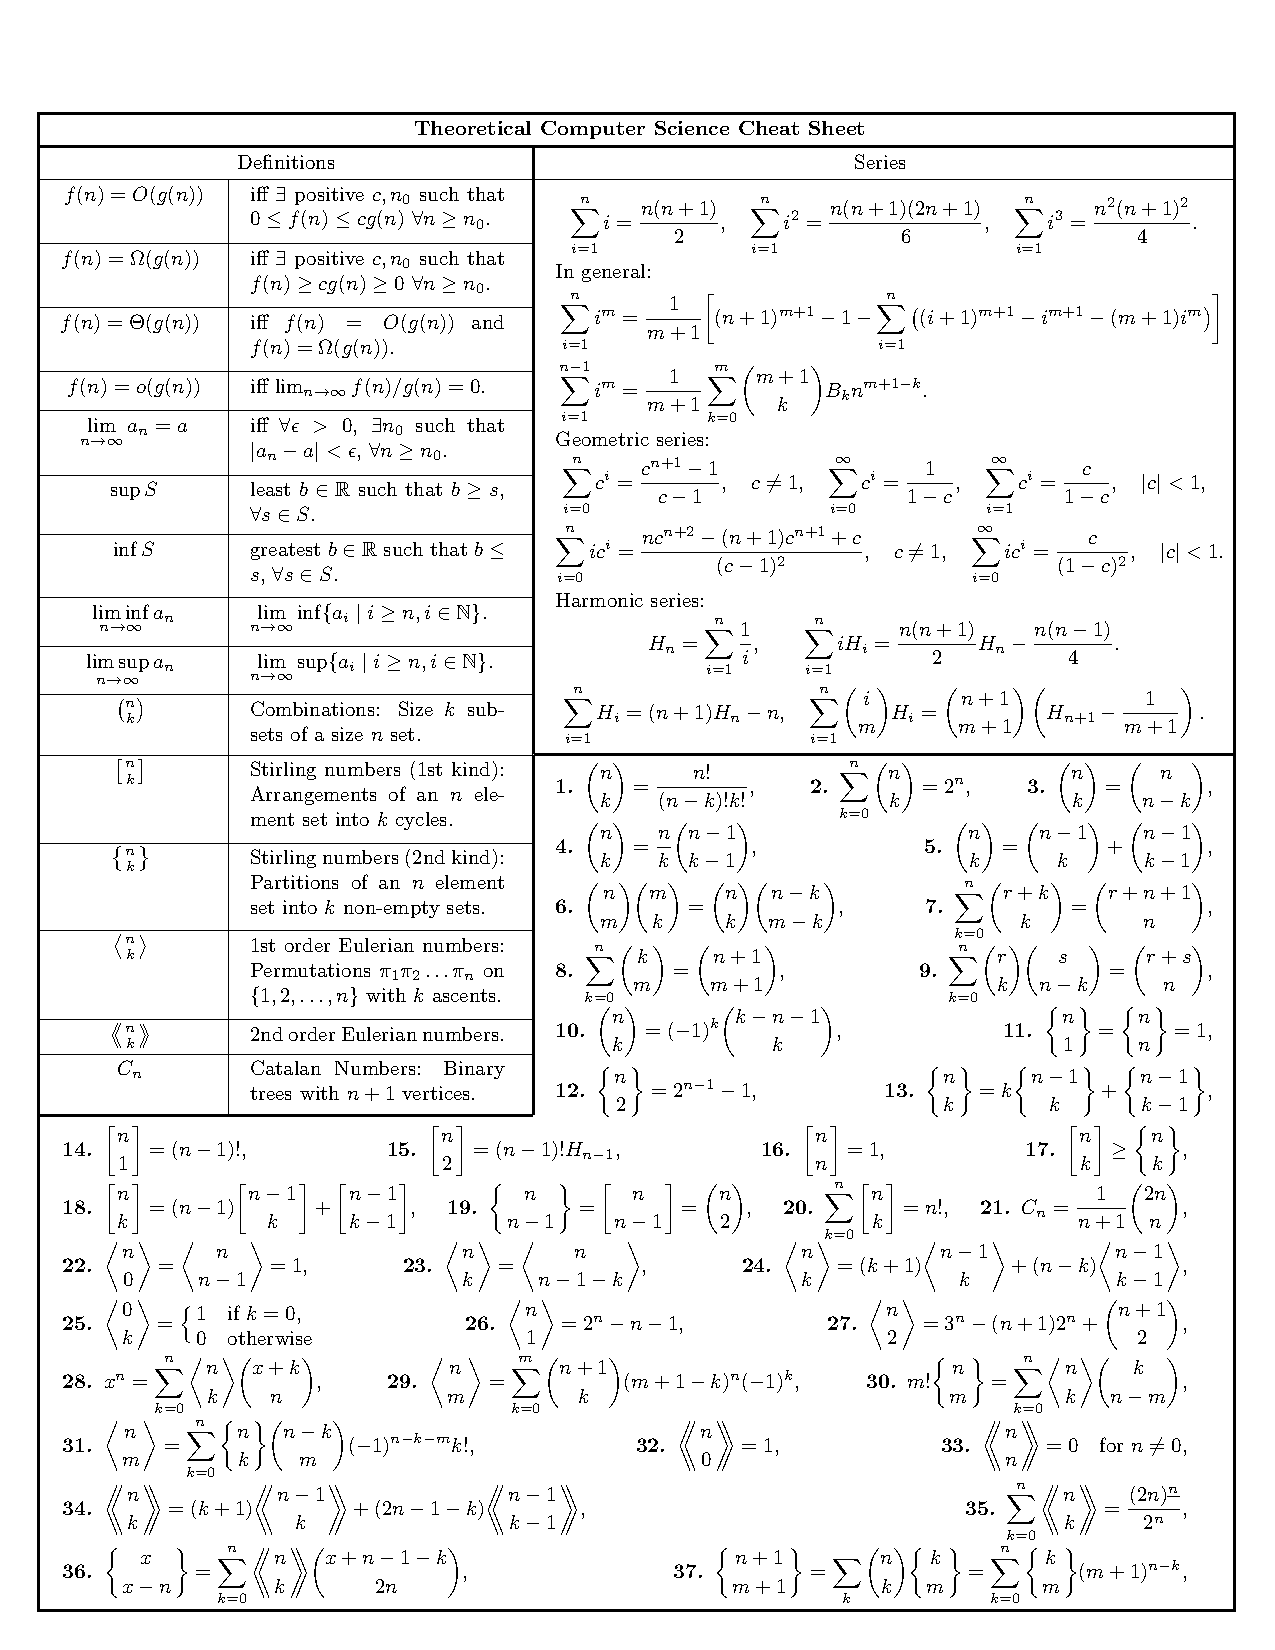
\includepdf[pages=-]{cheat.pdf}

%\newpage
%\section{Others}

\end{document}
